\documentclass[border=0.5mm]{standalone}

\usepackage{import}
\subimport{../../../}{preamble.tex}

\usepackage{tikz}
\usetikzlibrary{calc}

\usepackage{pgfplots}
\usepgfplotslibrary{fillbetween}

\begin{document}

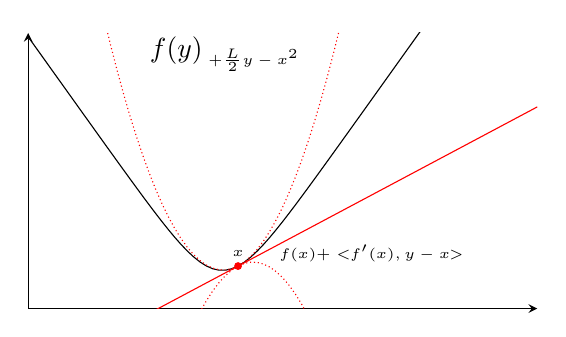
\begin{tikzpicture}

  \begin{axis}[
    ticks=none,
    axis lines=left,
    y=0.7cm,            % y unit vector
    x=1cm,            % x unit vector
    clip=true,
    ymax=5,
    ymin=0,
    % xlabel={ $\Re^n$},
    ylabel={ $f(y)$},
    x label style={at={(axis description cs:0.8,0.05)},anchor=west},
    y label style={at={(axis description cs:0.22,0.85)},rotate=-90,anchor=south west},
    ]
    
    \addplot[mark=none, black, samples=100, domain=-4:4] { ln(exp(2*x) + exp(-2*x)) };

    \addplot[mark=none, red, samples=100, domain=-4:4] { ln(exp(2*0.2) + exp(-2*0.2)) + (x-0.2)*0.759898 };
    \node[right] at (axis cs:0.6, 1) {\tiny \red{$f(x) + <\!\!f'(x), y-x\!\!>$}};

    \addplot[densely dotted, mark=none, red, samples=100, domain=-4:4] { ln(exp(2*0.2) + exp(-2*0.2)) + (x-0.2)*0.759898 + 4/2*(x-0.2)^2 };
    \node[right] at (axis cs:-0.3, 4.5) {\tiny \red{$+\frac{L}{2}\norm{y-x}^2$}};
    
    \addplot[densely dotted, mark=none, red, samples=100, domain=-4:4] { ln(exp(2*0.2) + exp(-2*0.2)) + (x-0.2)*0.759898 - 4/2*(x-0.2)^2 };

    %\node[right] at (axis cs:-1, 4.75) {\tiny \red{$\dots + \tfrac{L}{2} \norm{y-x}^2$}};

    \node[circle, inner sep=1, fill=red] (x) at (axis cs:0.2, 0.771101) {};
    \node[above] at (x) {\tiny \red{$x$}};
  \end{axis}
  
\end{tikzpicture}

\end{document}

%%% Local Variables:
%%% mode: latex
%%% TeX-master: t
%%% End:
